\documentclass[dvipdfmx, 12pt]{article}
\usepackage{mathpazo}
\usepackage{amsmath,amssymb}
\usepackage{array}
\usepackage[hiresbb]{graphicx}
\usepackage{tikz}
\usepackage{textcomp}
\usepackage{dcolumn}
\usepackage{here}
\usepackage{lscape}
\usepackage[top=25truemm,bottom=30truemm,left=25truemm,right=25truemm]{geometry}
\begin{document}

\title{Reference Dependence and Monetary Incentive \\
-Evidence from Major League Baseball-}
\author{Reio Tanji}
\date{}
\maketitle

\leftskip = 25pt
\rightskip = 25pt
  \small
  \textit{
  Many empircal studies have revealed the existance of reference-point dependent preference in field settings, including cases from professional sports players' decision making, whose performance is observed by the manager and evaluated. If there is some incentives that leads the individuals take ``apparent'' reference point dependent behaviror, then we should rather think it is reference dependence of the managers that evaluates the players.. In this paper, I picked up the case of Major League Baseball players, which Pope and Simonsohn (2011) reported have reference-point dependent tastes about the number of their batting-average. I first confirmed the evidences that supports reference point dependent manipulation of batting-average and other performance indexes. Then I tested if there exist any monetary incentives that encourage the players to do so. My results are against this assumption: no overestimation of achieving the possible reference point was observed, which confirms that players adjust their aspiration level to reach their internal goal, even though there is no additional bonus that rewards their achievement.
  }



\leftskip = 0pt
\rightskip = 0pt
\normalsize


\section{Introduction}

Reference-point dependence is one of the most important concepts to evaluate outcome, and it affects the agents' following economic behavior. Classical economic models assume that economic agents evaluate choice/prospects according to abolute value of (expected) return. On the other hand, Tversky and Kahneman (1992) introduced behavioral assumption: reference-point dependent preference sets some target value of the outcome and then subjects regard the possible outcome as gain or loss from the target. For example, workers feel happy if her/his wage goes up to \$15 per hour, but vice versa if it goes down to \$15, although the absolute value of \$15 is actually same. In this case, s/he evaluates their new wage with the reference point of the previous one.

Prospect theory, which is advocated by Tversky and Kahneman, consists of two main charactaristics: one is probability weighting function, and the other is reference dependence, mentioned above. It enabled us to interpret cases that seems inconsistent with the traditional economic theory, and made it possible to understand them with some additional assumptions. Thus, a lot of following researches conducted in field settings or laboratories.

Reference dependence is also observed in the behavior of athletes. Pope and Schweizer (2011) found that professional golf players regard ``per,'' the standard number of shots determined according to the difficuly of each hole, as reference points. Also, Pope and Simonsohn (2011) tested the existance of the reference dependence in the Major League Baseball, a professional baseball league of America.  When dealing with the case of the professional athletes, however, we must pay attention to how their salary contract is designed.

Suppose the case of the professional golf player. Golf is essentialy competition of the total number of shots they needed to finish the whole tour, regardless of that of each single hole, or whether s/he saves per or not in the hole. Rank of order is determined according to this number, and those with better scores are rewarded. Then, what about when there is some monetary incentive to make effort to save per? That is, if every time s/he saved per in each hole, then s/he can get some additional bonus separated from their total score. In this case, then, making effort to save per can be interpreted as sufficiently ``rational'' choice, although the observed behavior itself appears to be evidence of the reference dependence.

In this paper, I picked up the evidence from Major League Baseball (MLB) position players' behavior following Pope and Simonsohn (2011), and considered the questions above. First, I specified the existance of some ``apparently'' possible behavior that shows reference point dependent preference of them. Then, I tested if this manipulation is in fact pursued from the player`s reference point dependent preference.

MLB position players seems to have some reference points, about their batting performance indexes: .300 of batting average is one of the possible ones. Pope and Simonsohn (2011) have shown, that there exists bunching just above .300 of the distribution of this index. As a required premise, I first tested if there is any evidence for the manipulation around the round numbers, not only .300 of batting average, both for other points of batting-average and other indexes, such as homerun or stolen-bases. The result supported the previous study and there observed similar tendency in some of other ones.

Confirming this, then I made examinations to answer the question, ``Is this observed manipulation truly driven by the reference dependence of the players?'' It is true that there exists bunching just above the possible reference points, but it is not sufficient yet, since team managers assign some incentives for the players to adjust their aspiration level to meet those points. I applied regression analysis using the data of the players` salary, and revealed that there does not exists such an incentive for them: Observed behavior is actually the reference dependence of the players. I also consulted other methodologies and evidences to confirm these ways also drew essentialy same results. Furtheremore, I submit other probability that is not confirmed due to lack of data, then conclude the paper.

This paper proceed as follows. In the Section 2, I review some literature and verify the standpoint of my paper. Section 3 describes the data I availed. Section 4 presents theoretial framework and empirical way to specification, and make some conjecture.  Section 5 show the results of the analysis. Discussion about some alternative interpretation and non-statistical data are included in Section 6. Finally, Section 7 concludes the paper.

\section{Literature Review}

  Tversky and Kahneman (1992) mentioned reference point dependence as one of the two distinct respects of their prospect theory. The most primitive form of reference dependent utility function is:

   \[
  u(x | r) = \begin{cases}
  x - r & \text{ if }x \geq r \\
  \lambda (x - r) & \text{ if }x < r
\end{cases}
  \]
  where $x$ denotes a certain outcome, and $r$ is one of the reference points. This agent evaluates the outcome by the difference from the reference point. In adiition, they assume ``loss-aversion'' of the individual, or $\lambda > 1$. Those who have this type of utility function, than they regard same absolute amount of outcome in different way, depending on s/he faces gain or loss situation. ``Diminishing sensitivity,'' which is concave in facing gain and convex in facing loss is an advanced form of this specification.

  Diecidue and Van de Ven (2008)`s ``aspiration level'' model added discontinuity assumption: that is, a utility function that ``jumps'' at the reference point. When ther exists jump in their utility function, then individuals try to manipulate outcome level, paying addtional cost which was not accepted in the standard ``smooth'' form of utility function. As mentioned below, I exploit this assumption to my model in this paper.

  \begin{tabular}{ccc}
    \begin{minipage}[H]{0.3\textwidth}
      \begin{figure}[H]
        \begin{tikzpicture}
          [domain = -2:2, samples = 200, >= stealth]
          \draw[->] (-2,0) -- (2,0) node[right]{$x$};
          \draw[->] (0,-2) -- (0,2) node[above]{$u(x)$};
          \draw plot[domain = 0:1.7] (\x, \x);
          \draw plot[domain = -0.9:0] (\x, {2 * \x});
          \draw (0,0) node [below right] {$r$};
        \end{tikzpicture}
        \scriptsize
        \caption{primitive gain-loss function}
        \label{gain-loss}
      \end{figure}
    \end{minipage} &
    \begin{minipage}[H]{0.3\textwidth}
      \begin{figure}[H]
        \begin{tikzpicture}
          [domain = -2:2, samples = 200, >= stealth]
          \draw[->] (-2,0) -- (2,0) node[right]{$x$};
          \draw[->] (0,-2) -- (0,2) node[above]{$u(x)$};
          \draw plot[domain = 0:1.7] (\x, {sqrt( \x)});
          \draw plot[domain = -1.7:0] (\x, {-sqrt(2 * - \x)});
          \draw (0,0) node [below right] {$r$};
        \end{tikzpicture}
        \scriptsize
        \caption{diminishing sensitivity}
        \label{dim-sen}
      \end{figure}
    \end{minipage}&
    \begin{minipage}[H]{0.3\textwidth}
      \begin{figure}[H]
        \begin{tikzpicture}[domain = 0:4, samples = 200, >= stealth]
          \draw[->](-0.5, 0) -- (4.2, 0) node[right]{$x$};
          \draw[->](0, -0.5) -- (0, 3.7) node[above]{$u(x)$};
          \draw[-](2.2, -0.1) -- (2.2, 0.1);
          \draw[domain=0:2.2,samples=200,>=stealth] plot (\x, {sqrt(\x)});
          \draw[domain=2.2:4.1,samples=200,>=stealth] plot (\x, {sqrt(\x) + 0.8});
          \draw (0, 0) node[below left]{O};
          \draw (2.2, -0.3) node {$r$};
        \end{tikzpicture}
        \scriptsize
        \caption{jump at the reference point}
        \label{jump}
      \end{figure}
    \end{minipage}
  \end{tabular}

  \vspace{1zw}

  Individuals with such reference-point dependent utility try to adjust their effort level so as to achieve their internal target, or reference point. There are a number of empirical literature that specifies the existence of reference dependence in the field or lab studies. Farber(2008) applied this model to the labor supply of New York cab drivers to show that as soon as they reached daily target sales, they considers to quit, even when they reached it early in each day. Jones(2018) made analysis on the system of American tax payment. He showed that individuals try to manipulate their real payment by substituting it by donation or other charitable action, and that especially when facing losses, they make more effort. This observation is also caused loss-aversion, with the reference point of zero-payment threshold.

  Reference dependence also occurs in the cases of sports. One of the most well-known papers amoung them is Pope and Schweizer (2011). They obtained the data of professional golf players, to point out that in each hole, players behave as they take ``per'' as the reference point: Specifically, they scceeed their putts, significantly better when the putt was one to save per than when it was one to get ``eagle'' or ``birdie.'' Similarly, Allen \textit{et al} (2016) specified the existance of reference point dependence of marathon runners, using data about the finish time of enormous number of race in the United States. In this case, the distribution of finishing time has excess mass around evry hour and 30 minutes. Note that these cases are common in that even if they achieve their internal goals, they do not receive any monetary reward for their success. Professional golf players are awarded according to the total number of shots through the whole tour, not to the number of pers they saved.
  %注釈:サブ4で特別な表彰?

  Pope and Simonsohn (2011) mention a seemingly similar case. They picked up three empirical evidence of round number as reference points: SAT (a standardized test for college admission in the United States) scores, laboratory experiment, and baseball. In their section of baseball, they picked up the evidence of Major League Baseball (MLB) players to claim that they suggest their reference depenent preference by the distribution of their perfonmance index: batting-average (AVG). According to their paper, the position players (batters) pay attention to their batting-average (AVG), especially to finish each season with their batting average of just above .300. They obatined MLB season individual AVG data from 1975 to 2008 and observed position players (= players except for pitchers) with at least 200 at-bats in each season. Then, they found that their distribution of the batting-average has excess mass just above .300, which reveals the existance of manipulation there.Furthermore, they found that players with batting-average of just below .300 are more likely to hit a base-hit and less likely to get a base-on-balls. Both base-hits and base-on-balls avoid the batter from being gotten out, so for the team he belongs to, base-on-balls also have important value to win the game. However, batting-average does not count base-on-balls as the element to raise the number (For the definition of performance statistics, see Appendix), so they prefer getting hit to base-on-balls. Thus, observed behavior they claims is sufficient evidence that shows the existance of round-number reference point dependent preference of the MLB players.

  It is true that there is observed behaviror similar to the cases of Pope and Schweizer (2011) or Allen \textit{et al} (2016). However, one important thing we have to take care of is there exists procedure of contract between the player and the team manager: those who evaluate the player. In other words, it may owe to their monetary value function, not by the preference of themselves. This is the main contribution of my research.

  Pope and Simonsohn stated in their own paper that they conducted analysis only for batting-average, and following research is to be made. So I first follow this: ``Is batting-average unique case?'' Then, I test if there exists monetary incentive for the player. If the team managaers they belong to adopt a system of salary that discontinuously ``jump'' by a certain performance index reaching to the point where manpulation is observed, then for the players it can be interpreted as rational choice, given the contract design. In general, players with their performance index just above these cutoff point and those just below the point have almost same ability as a baseball player. At least, it is natural to think there is no reason to treat players discontinuously better, only because he achieve the cutoff. Then, it is interpreted that it is rather the team manager than the players themselves who have the reference-point dependent preference, which makes the players encouraged to meet their goals.

  On the other hand, if there exists no evidence that team managers evaluate the players by the achievement of the cutoff, then we can say that the observed behavior is truly drawn by their own reference dependence. In addition, the consistency is so strong that even there exists no rational reason, they try to reach there. Analysing this and verify which hypothesis is my main contribution of this paper.

\section{Data Description}

In order to make empirical research, I need information about players' performance, contracts and other details. Then, I generated panel data that contains these specific information from some open data-source. Each sample is obtained by unit of a single season, but due to lack of open source of information about countracts, time range of the data used in each analysis is unbalanced.

Performance are obtained obtained from baseball fan website:  \textit{fangraphs} and \textit{Baseball Reference}. Since the regulation of ``qualified plate-appearances,'' the cutoff number to get batting title such as batting-average, was introduced in 1957, I collected dataset from this year. Stats in each season contains that of only during the regular season, not that of Spring-Training or postseason games. The full-sample is $N=54469$.

Salary data are obtained from American media site: \textit{USA TODAY}. I collected salary data of the position players who are registered in MLB Roaster at the beginning of each season, and merged with the play stats in the previous year, because salary is as usually determined based on the performance of the previous season. Data was available only that since 1987, and as I need data of the next year about the salary, latast season is 2017. The aggregated number of the panel is $N=13226$.

Then, for precise research, I made some sample-restriction. First of all, I have to distinguish the data with both play stats and contract, with that with only play stats. In section of specifying excess mass, I utilize the latter one (I call this Sample A), and in analyzing the monetary incentive, I use the former one (Sample B).

In considering rate indexes, we have to restrict the sample to the batters with a certain number of attendances, since these indexes of those with too little at-bats are enormously affected by the result of every single plate-appearances, and so team managers might not see them in evaluating performance. At Pope and Simonsohn (2011), the threshold was set at 200 at-bats, but in my research, I substitute at-bats with plate-appearances, since at-bats exclude the plate appearances with base-on-balls and hit-by-pitch, even though they attended the game and appear to the plate. Restricting the sample to the players with at least 200 plate-appearances yields $N=18143$ for Sample A and $N=8915$ for Sample B.

Play stats are tagged by players` ID and season, including batting indexes tested bunching: batting-average, on-base percentage, base-hits, stolen-base, homerun, runs-batted-in, and plate appearances. Moreover,  for the analysis of monetary incentives, I collected other indexes that control the performance: slugging-average, OPS, fWAR, BATTING, FIELDING, BaseRun, and WPA. Salary data includes annual salary at the year: for the players with plural-year contract, it is calculated by deviding total payment of the contract by the years. It also contains the player-specific charactaristics: age, position (catcher, firstbaseman, ... right fielder), team they signed, and possession of the right of free agency.

The summery statistics are descripted in Table \ref{sum_A} and Table \ref{sum_B}.

\begin{table}
  
% Table created by stargazer v.5.2.2 by Marek Hlavac, Harvard University. E-mail: hlavac at fas.harvard.edu
% Date and time: ��, 11 08, 2018 - 14:34:36
% Requires LaTeX packages: dcolumn
\begin{table}[H] \centering
  \caption{Summary Statistics for Sample A}
  \label{sum}
\scriptsize
\begin{tabular}{@{\extracolsep{1.2pt}}lD{.}{.}{-3} D{.}{.}{-3} D{.}{.}{-3} D{.}{.}{-3} D{.}{.}{-3} D{.}{.}{-3} D{.}{.}{-3} }
\\[-1.8ex]\hline
\hline \\[-1.8ex]
Statistic & \multicolumn{1}{c}{N} & \multicolumn{1}{c}{Mean} & \multicolumn{1}{c}{St. Dev.} & \multicolumn{1}{c}{Min} & \multicolumn{1}{c}{Pctl(25)} & \multicolumn{1}{c}{Pctl(75)} & \multicolumn{1}{c}{Max} \\
\hline \\[-1.8ex]
PA & 18,143 & 456.477 & 152.836 & 200 & 320 & 591 & 778 \\
HR & 18,143 & 11.811 & 9.747 & 0 & 4 & 17 & 73 \\
RBI & 18,143 & 51.882 & 26.912 & 4 & 31 & 69 & 165 \\
SB & 18,143 & 7.846 & 10.869 & 0 & 1 & 10 & 130 \\
AVG & 18,143 & .264 & .032 & .135 & .242 & .285 & .394 \\
OBP & 18,143 & .331 & .039 & .174 & .305 & .356 & .609 \\
Age & 18,143 & 28.506 & 4.042 & 18 & 25 & 31 & 46 \\
H & 18,143 & 108.941 & 42.933 & 29 & 72 & 143 & 262 \\
OPS & 18,143 & .738 & .106 & .382 & .665 & .805 & 1.422 \\
\hline \\[-1.8ex]
\end{tabular}
\end{table}

\end{table}

\leftskip = -15pt
\begin{table}
  
% Table created by stargazer v.5.2.2 by Marek Hlavac, Harvard University. E-mail: hlavac at fas.harvard.edu
% Date and time: ��, 11 08, 2018 - 14:49:25
% Requires LaTeX packages: dcolumn
\begin{table}[H] \centering
  \caption{Summary Statistics for Sample B}
  \label{sum_B}
\scriptsize
\begin{tabular}{@{\extracolsep{-5pt}}lD{.}{.}{-3} D{.}{.}{-3} D{.}{.}{-3} D{.}{.}{-3} D{.}{.}{-3} D{.}{.}{-3} D{.}{.}{-3} }
\\[-1.8ex]\hline
\hline \\[-1.8ex]
Statistic & \multicolumn{1}{c}{N} & \multicolumn{1}{c}{Mean} & \multicolumn{1}{c}{St. Dev.} & \multicolumn{1}{c}{Min} & \multicolumn{1}{c}{Pctl(25)} & \multicolumn{1}{c}{Pctl(75)} & \multicolumn{1}{c}{Max} \\
\hline \\[-1.8ex]
Age & 8,915 & 28.714 & 3.901 & 19 & 26 & 31 & 46 \\
PA & 8,915 & 471.946 & 150.890 & 200 & 342 & 605.5 & 778 \\
AVG & 8,915 & .268 & .031 & .146 & .248 & .289 & .394 \\
OBP & 8,915 & .337 & .038 & .174 & .311 & .360 & .609 \\
HR & 8,915 & 13.446 & 10.213 & 0 & 6 & 19 & 73 \\
RBI & 8,915 & 56.339 & 27.621 & 5 & 35 & 74 & 165 \\
SB & 8,915 & 8.534 & 10.851 & 0 & 1 & 11 & 109 \\
H & 8,915 & 114.232 & 42.481 & 30 & 78 & 148 & 262 \\
+WPA & 8,915 & 8.715 & 3.471 & 2.030 & 5.820 & 11.430 & 19.160 \\
-WPA & 8,915 & -8.270 & 2.610 & -15.050 & -10.420 & -6.060 & -2.740 \\
Bat & 8,915 & 3.257 & 16.139 & -44.200 & -7.300 & 11.100 & 116.800 \\
Fld & 8,870 & .304 & 7.482 & -36.100 & -4.000 & 4.400 & 37.000 \\
BsR & 8,915 & .092 & 2.712 & -12.600 & -1.200 & 1.200 & 14.300 \\
Salary & 8,915 & 3,487,838 & 4,487,344 & 62,500 & 512,750 & 4,658,334 & 29,200,000 \\
FA & 8,915 & .168 & .374 & 0 & 0 & 0 & 1 \\
\hline \\[-1.8ex]
\end{tabular}
\end{table}

\end{table}
\leftskip = 0pt

\section{Theoretical Frameworks and Way of Specification}

\subsection{Frameworks}

MLB position players try to maximize their performance, for two main goals: one is to contribute to their team winning more games, and the other is to improve their living standard. That is, getting better contract and playing as long as possible is one of the most important object to play for the team. Performance index is clear and valid benchmarks to signal their ability to the team managers. Baseball is so rich in such indexes, so we can say these are good reliable proxy for their ability as a player. We assume a utility function of the player/manager as $u(x)$ for the value of a certain index $x$. Players' self-evaluation and his salary for the next season reflects this value.

Then, here I describe the nature of the indexes. Baseball batting indexes are roughly divided into two types. One is that simply indicates the number of a ceratain plays, and another is calculated using these numbers. Here I call the former ``cumulative index,'' and the latter ``rate statistics.'' Cumulative index are for example ``base-hit'' or ``homerun,'' or ``stolen-bases.'' They are irreversible and so once they reach a certain number then it cannot be decrease. On the other hand, rate indexes can be fluctuate, so in order to keep this kind of indexes above their goal, they have to continue to make effort or stop attending game and wait for the end of the season. Batting-average is sorted of this type, and On-base percentage or OPS are also kind of them. Note that even though I call this for ``rate'' index for simplisity, it contains all the index that can both go up and down according to the player's performance, such as OPS or slugging-average. See Appendix for specific definition of each index.

Anyway, the important assumption is that players evaluate their performance index using referene-dependent utility function of themselves or the team manager, and manipulate it in order to maximize their utility. This aspiration results in odd distribution of the index at the end of the season: excess mass around the possible referene point. In this paper, following Allen \textit{et al} (2016), I exploit the assumption of the utility function of Diecidue and Van De Ven (2008)`s ``aspiration level" model. The model presents the form of the utility function with ``notch,''

\[
\lim_{\epsilon \to 0} v_r (r + \epsilon) \neq
\lim_{\epsilon \to 0} v_r (r - \epsilon)
\]
This form of utility function is discontinuous at the reference point $r$.

In my paper, it is not determined who has such a utility function. At least one of the these two agents: players and managers has reference dependent feature in their utility. Players pay attention to if each index are above the reference points.In  Allen \textit{et al} (2016), it is assumed that discontinuous utility function occurs as excess mass around the reference points. In my paper, I suppose there may be another story. That is, discontinuous utility function of the managers emerges as discontinuous evaluation of the players: salary scheme jumps, depending on whether a ceatain performance index is above or below the reference point. Then, it modifies the income function of the players discontinuous, which results in bunching as the best response of them.

 \subsection{Empirical Method}

  \subsubsection{Test for Bunching}

  First, I test if there is observed any behavior that seems to be related to reference dependent preference. As I explained in the previous chpaters, the existance is verified by the observation of bunching, or excess mass around the possible reference point. To specify the excess mass, I apply the method of regression discontinuity design (RDD).

  RDD is a way to measure the effect of a treatment, such that whether the treatment is assigned or not depends on the threshold of a certain variable (called ``running variable''). Then, comparing the samples just above and just below the threshold is sufficient examination of the treatment, since they are in almost same states except for the existance of the treatment.

  However, there is an important assumption for this specification to be valid (Lee and Lemieux, 2010): continuity of the running variable around the threshold. In other words, individuals must not be able to manipulate the running variable so as to be above the cutpoint. This is because if there exists manipulation, then there occurs selection bias problem, that those who try to be assigned the treatment can adjust their running variable. Therefore, there are some empirical way to test the manipulation of a variable, which is the very method I apply in my analysis.

  One of the frequently applied methods for this specification is  McCrary(2008)'s local linear density estimation. I avail this to my specification of bunching.

  This estimation of the manipulation at the cutoff point $c$, proceeds in two steps: undersmoothing histograms and local linear smoothing. Undersmoothing means to determine the binsize $b$ of the running variable: in this paper, the index argued.

  \[
  g(R_i) = \left \lfloor \dfrac{R_i - c}{b} \right \rfloor b
  + \dfrac{b}{2} + c \in \left \{ \ldots, c-5\dfrac{b}{2},  c-3\dfrac{b}{2}, c-\dfrac{b}{2}, c+\dfrac{b}{2}, c+3\dfrac{b}{2}, c+5\dfrac{b}{2}, \ldots \right \}
  \]
  where $\lfloor a \rfloor$ denotes the greatest integer less than $a$, and $g(R_i)$ stands for the height, or frequency of each bin. Then, we make local approximation above and below $c$, the possible value of reference dependence point. Bandwidth is calculated to minimize the estimation error. Then, we estimate the frequency at the cutoff point, $\Hat{f}(r)$, by fitting the estimated density function below and above the cutoff, $\hat{f}^+$ and $\hat{f}^-$, respectively. Finally, we take the difference between $\ln \hat{f}^+$ and $\ln \hat{f}^-$ to calculate the statistics $\theta$. With $\theta$ and its estimator of standard deviation, $t$-tests can be condtructed to specifying manipulation.

  \subsubsection{Monetary Incentive}

  Then, I examine the existance of the monetary incentive by regression analysis. The primitive model to check this is below:

  \[
  w_{it} = \beta_0 X_{it} + \beta_1 \text{ABOVE}_{it}
  + \beta_2 Z_{it}
  \]

  For each player $i$ in the season $t$, $w_{it}$ is log annual salary in next season $t+1$. $X_{it}$ and $Z_{it}$ are the value of performance index (batting-average, on-base percentage,\ldots) and other player-specific characters (age, team he signed, position,\ldots), respectively. $\text{ABOVE}_{it}$ is an indicator of the achievement of their goals for the index. That is, if he finished his season with a certain index with above the possible reference point, it takes 1, and otherwise 0. This is the variable in interest. As well as OLS, team, position, or individual fixed effect model estimation was also conducted.

  Also, to check the robustness of my analysis, I tried alternative methodology: include interaction term, and methodology of regression discontinuity design. Interaction term analysis include that of $X_{it}$ and $\text{ABOVE}_{it}$, the coefficient of which indicates additional return on their achievement. RDD method is simple sharp RDD method: local linear regression around the possible reference point as the cutoff, where the bandiwidth was selected according to the polynominal approximation (Imbens, Guido and Kalyanaraman, 2009). As I mentioned above, RDD can be invalid when individuals can manipulate the running variable, so this may not appropreate in this analysis since I confirm there exists manipulation in the running variable: performance index. However, as I show below, this analysis found no evidence of discontinuous design of contract. Therefore, I apply this result as a complimental evidence of my research.

\section{Result}
\subsection{Excess Mass Around The Reference Point}

First, I show the results that verifies bunching. Table \ref{Bunch-True} includes the summary of McCrary (2008)'s manipulation tests about the performance indexes that say there is some manipulation occurs. Consistent with Pope and Simonsohn (2011), there actually occurs excess mass around .300 of batting-average. Also, manipulation were also observed in some of other numbers of other indexes: .350 of on-base percentage, 20 of homeruns, 100 of runs-batted-in, 30 and 40 of stolen-bases, and 200 of base-hits. Table %\ref{}
shows parts of results that denies the existance of excess mass.

\begin{table}
  \small
  \centering
  \begin{tabular}{lcccccc}\hline
    index & type & cutpoint & binsize & bandwidth & $\theta$ & $z$
    \\ \hline \hline
    AVG & rate & .300 & .001 & .019 &  .499 & 7.442*** \\
    & & & & & (0.067) & \\
    OBP & rate & .350 & .001 & .024 &  .139 & 2.854** \\
    & & & & & (0.049) &  \\
    HR & cumulative & 20 & 1 & 5.309 & .259 & 3.465*** \\
    & & & & & (.075)  & \\
    RBI & cumulative & 100 & 4 & 15.423 & .311 & 3.295*** \\
    & & & & & (0.094) & \\
    SB & cumulative & 30 & 1 & 10.000 & .529 & 4.274*** \\
    & & & & & (.124) & \\
    & & 40 & 1 & 11.505 & .481 & 2.764** \\
    & & & & & (.174) & \\
    PA & cumulative & 500 & 1 & 0.003 & .160 & 2.515* \\
    & & & & &(.063) & \\
    H & cumulative & 200 & 1 & 18.922 & .453 & 2.547 * \\
    & & & & & (.178) & \\ \hline \hline
  \end{tabular}
  \footnotesize
  \flushright
      ***: $p<0.1\%$, **: $p<1\%$, *: $p<5\%$.

    Bandwidth is optimized following the method of Mcrary(2007).
  \caption{Test for Manipulation :leastPA $= 200$}
  \label{Bunch-True}
\end{table}

For batting-average, extending sample size from Pope and Simonsohn (2011) yields similar results: Players manipulate their batting-average. The difference between the estimated frequency according to the approximation below .300 and that of above .300 was significant at .1\% ($z=7.442$) level. Also, there were no other similar bunching points, even though it is a round number, .200, .250, or .350. The results are robust to changing the binsize of frequency.

On-base percentage, on the other hand, showed similar tendency in .350, although the significance level was $z=2.854$ (significant at 5\% level). Pope and Simonsohn (2011) reported that they are less likely to get base-on-balls when facing marginal range of batting-average and so they feel of more importance in batting-average than on-base percentage. However, when they face marginal point of on-base percentage, they may try to get more base-on-balls in order to achieve .350.

Bunching also occurs in cumulative indexes. Cumulative ones are irreversible, and so players may feel these indexes are easier to manipulate. As same as batting-average and on-base percentages, however, such manipulation was observed in only limited numbers: not all the round numbers. For Homerun ($z=3.465, p < 0.1\%$), bunching occurred only in 20: there may be diminishing sensitivity: 20 is located on above the 75 percentiles of the whole Sample A. Also, stolen-base and base-hit have shown bunching, at 30 ($z=4.274, p < 0.1\%$) and 40 ($z=2.764, p < 1\%$) of stolen-base and 200 in base-hit ($z=2.547, p < 5\%$). Stealing-bases are skill that are talented to limited number of the players, but succeeds with the prpbability of 60 to alomost 100 \%, so those who are evaluated by their number of stolen-bases, it may certain may be accessible number to manipulate. Base-hit is manipulated by similar to batting-average, but for this index, as same as other cumulative ones, it cannot be valid to be replaced in the last plate-appearance, which lower the confidence level of the $z$-statistics. And surprisingly such manipulation occurs in runs-batted-in. Compared to other indexes, runs-batted-in is harder to manipulate, since the number of that depends on the performance of his teammates, and the can earn at most 4 runs at a single plate-appearance. As in Table \ref{Bunch-True}, the test said that there occurs the evidence in plate-appearances. However, it may insufficient because the optimized bandwidth was smaller than one, even though the number of PAs takes only integers. Setting bandwidth larger than 1, then the result went insignificant.

\begin{figure}[H]

  \begin{tabular}{cc}
    \begin{minipage}{.5\textwidth}
      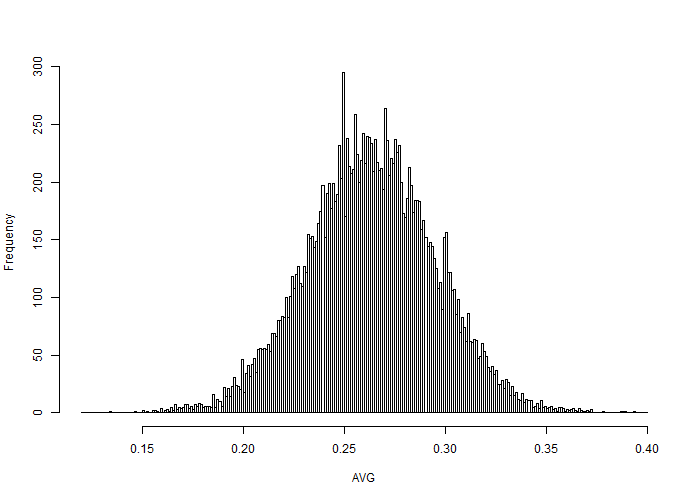
\includegraphics[keepaspectratio, scale = 0.5, angle=90]{graphs/hist_AVG_all.png}
      \caption{Histgram of Batting-Average}
      \label{hist_AVG}
    \end{minipage} &

    \begin{minipage}{.5\textwidth}
      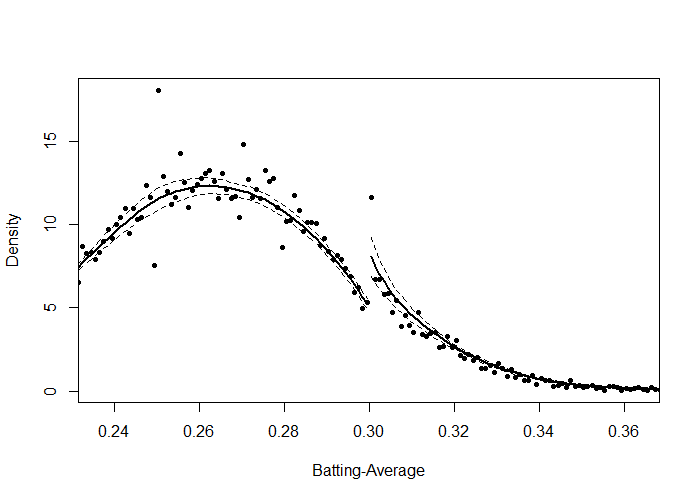
\includegraphics[keepaspectratio, scale = 0.65, angle = 90]{graphs/AVG_300.png}
      \caption{}
      \label{}
    \end{minipage}
  \end{tabular}
\end{figure}


\begin{figure}[H]
  \begin{tabular}{cc}
    \begin{minipage}{.5\textwidth}
      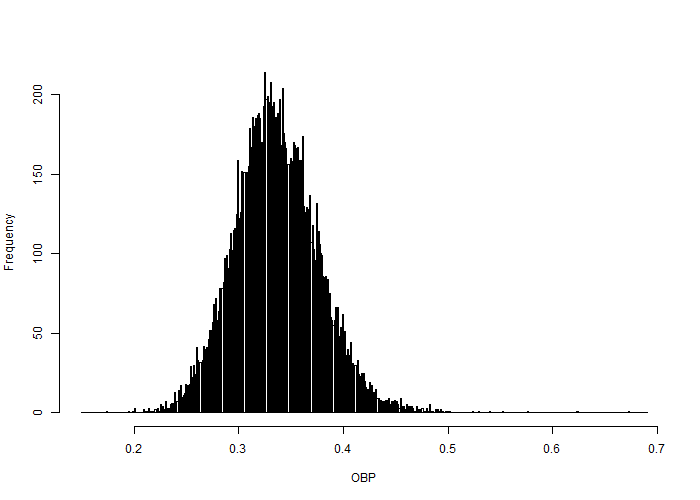
\includegraphics[keepaspectratio, scale = 0.5, angle=90]{graphs/hist_OBP_all.png}
      \caption{Histgram of On-Base Percentage}
      \label{hist_OBP}
    \end{minipage} &

    \begin{minipage}{.5\textwidth}
      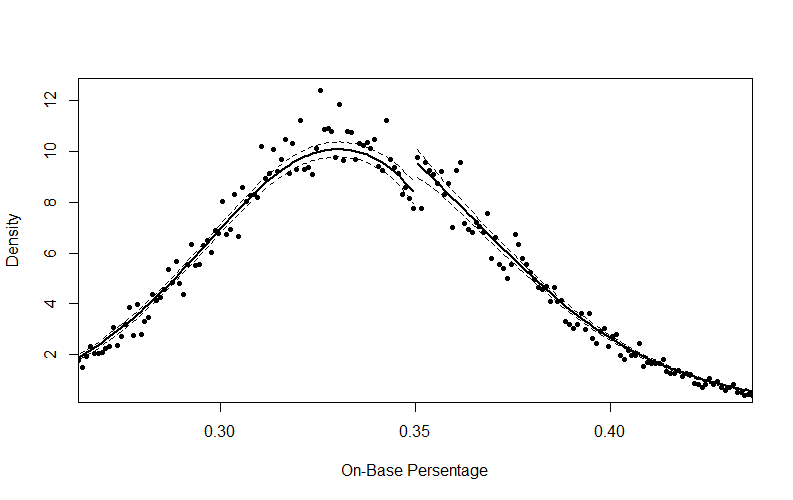
\includegraphics[keepaspectratio, scale = 0.5, angle = 90]{graphs/OBP_350.png}
      \caption{}
      \label{}

    \end{minipage}
  \end{tabular}
\end{figure}

\subsection{Existance of Monetary Incentive}

\section{Alternative Interpretation and Some Evidence}

In section 5, my analysis said that there in fact exists manipulation in some of the batting indexes, but no evidence observed in their contracts, which supports the assumption these observations are driven by the reference dependence of the players themselves. Here I consider some possible alternative and additional discussion about my result.

\subsection{Incentivised Contract}

One most possible explanation that may explain my result is the incentivised design of the contract.

\subsection{Misunderstanding by the Players}

Misunderstandings by the player is also a possible way to interpret the results.

\subsection{Contract Length}

Skilled players usually get contracts with plural-year package.

\subsection{By-Time Analysis}

My paper used data from wide range of time: 62 years for bunching, 31 years for monetary incentives. Through such a long time, techniques of the players or the quality of instruments must have evolved, which leads to change in mean or the standard value of the indexes. Also, it is natural to think there may have been a lot of change in the design of the contract they agreed. Here I consider time-variable elements in my analysis. specifically, there are two main possible effect that changes the contract design: one is the relative market power of the players, and another is change in relative importance of each performance index.

Relative market power has direct relation to the contract. Before the system of free agency was introduced, players are forbidden to move to other teams without permission by the team they belong to. `94 strike by the Players Association of Major League Baseball, against the team owners to request improvement of their treatment, also may have great influence on their contracts (See Appendix about the specific information about free agency and Strike).

Relative importance captures the change in evaluation of each index. Through the history of baseball, there have been invented a lot of indexes that measures the performance/ability of the player, and it has been argued which index is the best to evaluate them. One of the most important revoution was the publication of \textit{'Moneyball'}(2003), written by Michael Lewis. In this book, he described that batting-average is not as appropreate measure: there is more close correlation with total runs the team earns in the season in on-base percentage. In practice, Oakland Athletics applied strategy to form the menber of the team, and won the playoff. This story was widely spread and changed the sense of view about the baseball index. Then, one possible question occurs: ``Does the tendency of manipulation/discoutinuous contract design also change through the history of baseball?''

In this analysis, I replicate the methodologies conducted in the previous sections, but sorting the sample into periods below:

\begin{enumerate}
  \item Before Free Agency (1957 - 1975)

  \item After Free Agency and Before Strike (1986 - 1994)

  \item After Strike and Before \textit{Moneyball} (1995 - 2003)

  \item After \textit{Moneyball} (2004 - 2017)
\end{enumerate}



\subsection{Across Indexes: Priority of Manipulation}

\section{Conclusion}

This paper

\section{Appendix}

\subsection{Proxies for Performance}
\small

To measure batter's performance, I use some \textit{SABR Metrics}'s statistics. \textit{SABR} is short for \textit{Society of American Baseball Research}, an American organization of analysing baseball. They try to evaluate players in more ``efficient '' way,  or by statistics with more close correlation with the expected wins the team obtain.

\subsection{Important Events Related to Section 6.4}


\section{References}
\small
\begin{itemize}
  \item
\end{itemize}

\end{document}
